\documentclass[tikz,border=12pt]{standalone}
\usepackage{amsmath,amssymb}
\usetikzlibrary{calc,arrows.meta}

\begin{document}
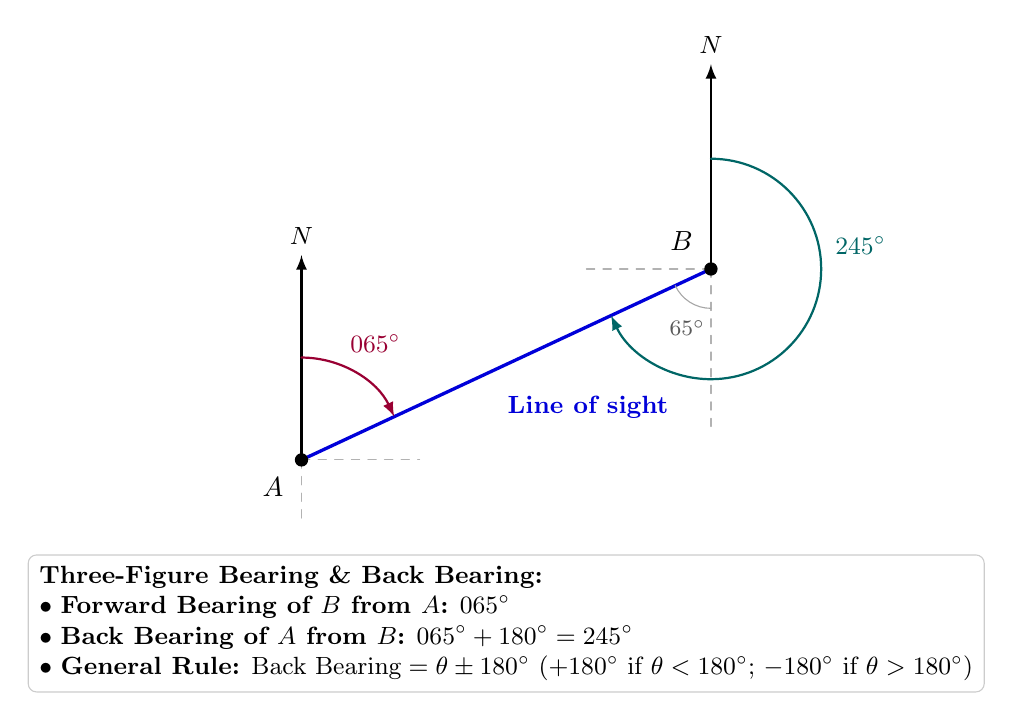
\begin{tikzpicture}[>=latex, line cap=round, line join=round]

  % Stations A and B
  \coordinate (A) at (0, 0);
  % Bearing 065 deg -> angle from positive x is 90 - 65 = 25 deg
  \coordinate (B) at (5.2, 2.425);

  % Connecting line of sight between stations A and B
  \draw[very thick, blue!85!black] (A) -- (B) node[pos=0.45, below right=4pt, font=\small\bfseries] {Line of sight};

  % --- Station A ---
  \draw[thick, ->] (A) -- ++(0, 2.6) node[above, font=\small\bfseries] {$N$};
  \draw[thin, dashed, gray!60] (A) -- ++(0, -0.8);
  \draw[thin, dashed, gray!60] (A) -- ++(1.5, 0);

  % Forward bearing arc at A (sweep clockwise 65 deg from North)
  \draw[thick, ->, purple!80!black] ([shift=(90:1.3)]A) arc[start angle=90, delta angle=-65, radius=1.3];
  \node[font=\small\bfseries, purple!80!black, fill=white, inner sep=1.5pt] at ($(A) + (57.5:1.75)$) {$065^\circ$};

  % --- Station B ---
  \draw[thick, ->] (B) -- ++(0, 2.6) node[above, font=\small\bfseries] {$N$};
  \draw[thin, dashed, gray!60] (B) -- ++(0, -2.0);
  \draw[thin, dashed, gray!60] (B) -- ++(-1.6, 0);

  % Back bearing reflex arc at B (sweep clockwise 245 deg from North to line BA)
  \draw[thick, ->, teal!80!black] ([shift=(90:1.4)]B) arc[start angle=90, delta angle=-245, radius=1.4];
  \node[font=\small\bfseries, teal!80!black, fill=white, inner sep=1.5pt] at ($(B) + (1.9, 0.3)$) {$245^\circ$};

  % Alternate interior angle arc at B (sweep clockwise 65 deg from South to line BA)
  \draw[thin, gray!70] ([shift=(-90:0.5)]B) arc[start angle=-90, delta angle=-65, radius=0.5];
  \node[font=\footnotesize, gray!70!black, fill=white, inner sep=1pt] at ($(B) + (-0.3, -0.75)$) {$65^\circ$};

  % Station points and labels
  \filldraw[black] (A) circle (2.2pt) node[below left=3pt, font=\normalsize\bfseries] {$A$};
  \filldraw[black] (B) circle (2.2pt) node[above left=3pt, font=\normalsize\bfseries] {$B$};

  % Explanatory Card / Summary below
  \node[align=left, font=\small, fill=white, inner sep=4pt, draw=gray!40, rounded corners=3pt, anchor=north] at (2.6, -1.2) {
    \textbf{Three-Figure Bearing \& Back Bearing:}\\
    $\bullet$ \textbf{Forward Bearing of $B$ from $A$:} $065^\circ$\\
    $\bullet$ \textbf{Back Bearing of $A$ from $B$:} $065^\circ + 180^\circ = 245^\circ$\\
    $\bullet$ \textbf{General Rule:} $\text{Back Bearing} = \theta \pm 180^\circ$ ($+180^\circ$ if $\theta < 180^\circ$; $-180^\circ$ if $\theta > 180^\circ$)
  };

\end{tikzpicture}
\end{document}
